\documentclass{article}
\usepackage{gensymb}
\usepackage{textcomp}
\usepackage{amsmath}
\usepackage{hyperref}
\usepackage{bookmark}
\usepackage{float} 
\usepackage{graphicx}
\usepackage{makeidx}
\usepackage[letterpaper, total={7.5in, 10in}]{geometry}

\makeindex
\begin{document}
\title{Potentials}
\author{Elias Xu}
\date{\today}
\maketitle
\setlength{\parindent}{0pt}

\tableofcontents


\section{Electrical Potentials}
Electric potentials are measures of the potential energy created by an electric field.
You can think of them as such:

\begin{center}
    Potential: Potential Energy :: Field: Force Energy
\end{center}
For the potential energy of point charges, there is a very big positional element here. As long as you have two charged particles, as long as they want to move somewhere, there will always be potential energy in that system. Usually, systems want to reduce that energy to zero.

\subsection{Formulas and Dimensional Analysis}
Let's look at the formulas for volts and field, and see what we can make for them. Let's have the formula for volts, and put of the formula for electric field for comparison.

\begin{align*}
    V = \frac{U}{q} &  & \vec{E} =  \frac{\vec{F}}{q}
\end{align*}

Let's do a quick dimensional analysis too for these \emph{volts}:

$$[V] = \frac{[J]}{[C]}$$

Differences between field and potential:

\begin{itemize}
    \item Field is a vector quantity, voltage is a scalar quantity
    \item Field lines are always perpendicular accross vector lines
\end{itemize}

Let's have a visualization changes of potential over time:

\begin{figure}[H]
    \centering
    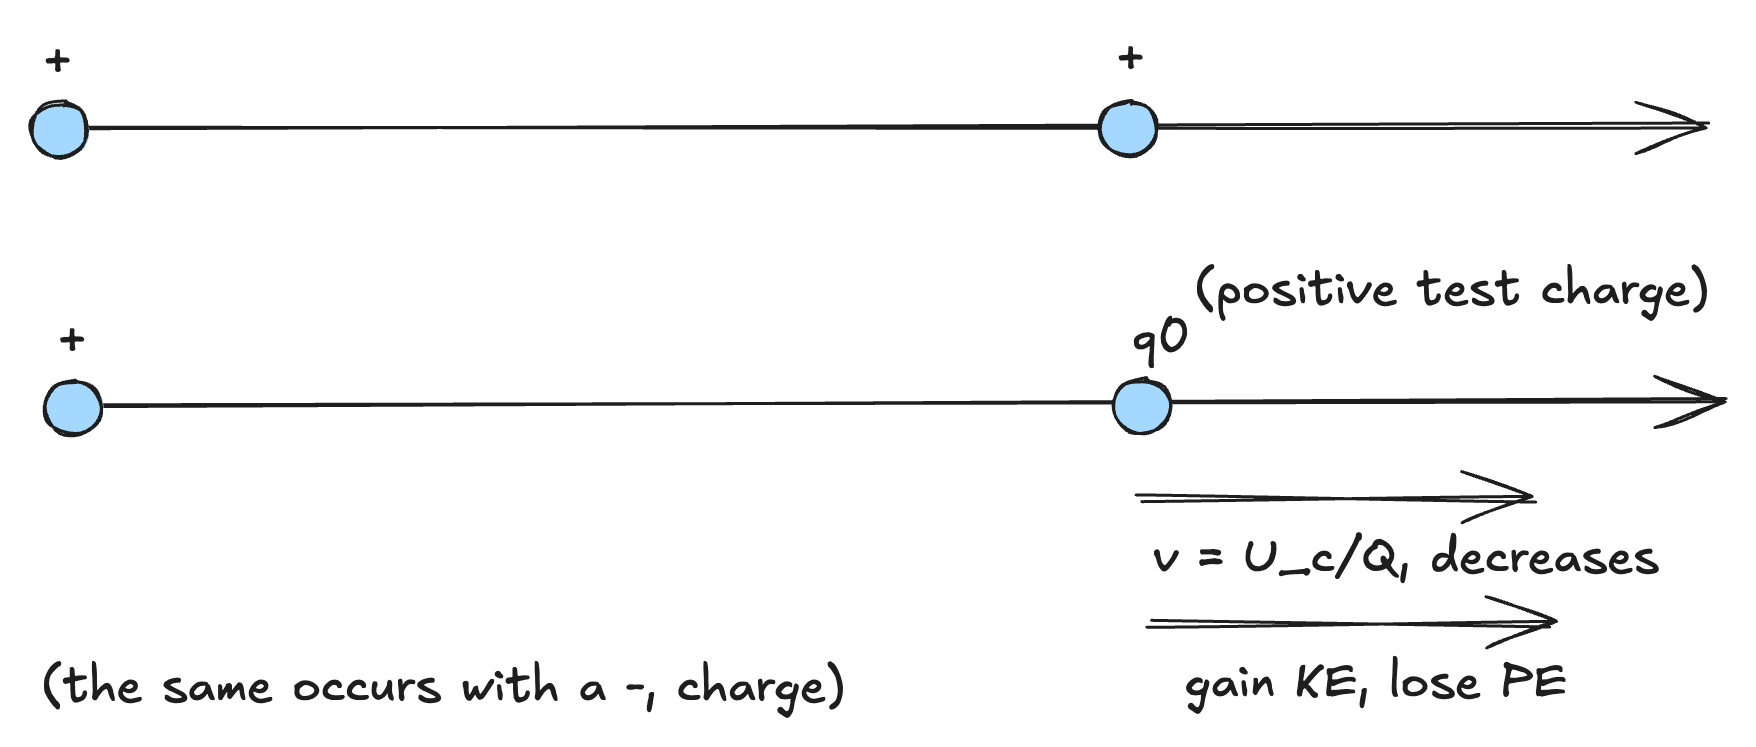
\includegraphics[width=0.5\textwidth]{figures/ChangeVAccrossNumberLine.png}
    \caption{The change of charge accross a number line}
\end{figure}

Notes:
\begin{itemize}
    \item Voltage decreases as one goes through a field lines
\end{itemize}

\subsection{Equipotentials}

\begin{figure}[H]
    \centering
    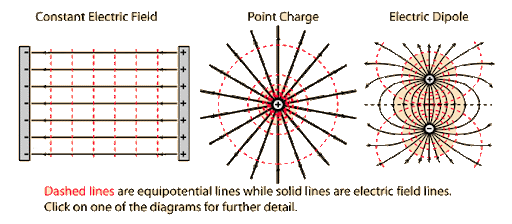
\includegraphics[width=0.5\textwidth]{figures/FieldvsPotentials.png}
    \caption{Example of electric fields vs electric potentials}
\end{figure}

\begin{itemize}
    \item Lines accross these show the areas of equidistant potentials
    \item Circular around point charge
    \item \emph{Perpendicular to field lines}, (e.g. Electric field is the negative gradient of potential), or $E = - \Delta V$
\end{itemize}

\subsection{Calculating Electrical Potential from Electric Field}
\begin{figure}[H]
    \centering
    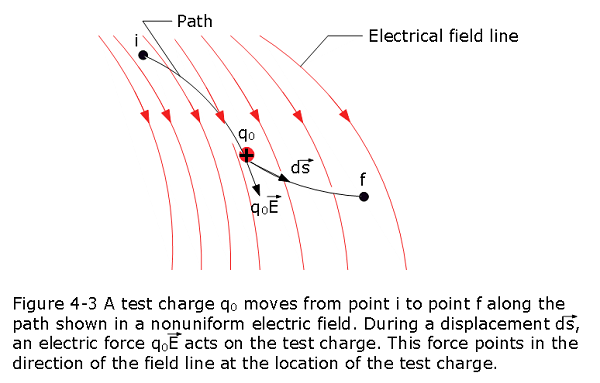
\includegraphics[width=0.5\textwidth]{figures/PotentialChanges.png}
    \caption{Visualization of the different differentials here}
\end{figure}

To try to find a formula for this, starting from the givens and working up.

\begin{align*}
    \vec{F} = q_0 \vec{E} &  & W = \int \delta W
\end{align*}

$$W = \int \delta w =  \int_{i}^{f} \vec{F} \delta \vec{s}$$
$$ = - \Delta U = - q_0 \Delta V $$
$$ \Delta v = \boxed{-\int_{i}^{f} \vec{E} \cdot \delta \vec{s}}$$

Given that electric field is a vector, and potentials are scalars, one might have to treat these as partial derivatives of x and y. So we have the original equation:

$$\vec{E} = \frac{Q}{4 \pi \epsilon R^2} = - \frac{\delta V}{\delta s}$$

But we have to split it into components:

\begin{align*}
    E_x = \frac{\delta V}{\delta x} &  & E_y = \frac{\delta V}{ \delta y} \\
\end{align*}

$$  \vec{E} = - \frac{\Delta V}{\Delta S} = \frac{\delta V}{\delta x} + \frac{\delta V}{\delta y}$$

\section{The Electic Potential of a Point Charge}

Given a ring of radius R, which has a uniformly distributed charge Q, we can infer the following:

\begin{itemize}
    \item The net electric field in the center is zero (common sense)
    \item The net electric field at every point is also zero (similar to gravatational field)
    \item What is the potential inside the ring, given $\Delta V = \int \vec{E} \cdot \delta \vec{s} = \int 0 \cdot \delta \vec{s} = \boxed{C}$.
\end{itemize}

\subsection{Calculating the Point Charge's Potential Through Integration}
Things to note:
\begin{itemize}
    \item Potential is a function of charge and radius, or the distance from a point
    \item Charge creates a scalar potential field
    \item $u(q_1, q_0) = q_0 V (q_1)$, the relationship between charge and potential energy
\end{itemize}

To get definite zero, we can set the potential at $r \to \infty$ to be zero, or $\lim_{r \to \infty} V(q) = 0$ to be zero.

$$\Delta V = V_f - V_i = 0 - V_i = \int_{r}^{\infty} \vec{E} \cdot \delta \vec{s}$$
$$- V_r = -\int_{r}^{\infty} \frac{1}{4\pi\epsilon_0} \frac{Q}{r^2} \left[\hat{r} \cdot \delta \vec{s}\right] = -\int_{r}^{\infty} \frac{1}{4\pi\epsilon_0} \frac{Q}{r^2} \delta r$$
$$\boxed{V_r = \frac{Q}{4\pi\epsilon r}}$$

Note that the property is \emph{scalar}. This makes stuff like addition and subtraction better!

\section{Electric Flux}
A measure of how many field lines pierces a certain surface / goes through a surface

\subsection{Finding formula for Electric Flux}
Flux is porportional to 
\begin{itemize}
    \item Cross sectional area of the surface [A]
    \item Strengh of the wires [E]
    \item orientation of the wires [$\theta$]
\end{itemize}

Max flux occurs when $\theta = 0 \degree$ (the angle between the normal of the surface and the field lines), and mix flux occurs when $\theta = 90 \degree$ (e.g. when normal of the surface and the field lines are perpendicular).

\begin{figure}[H]
    \centering
    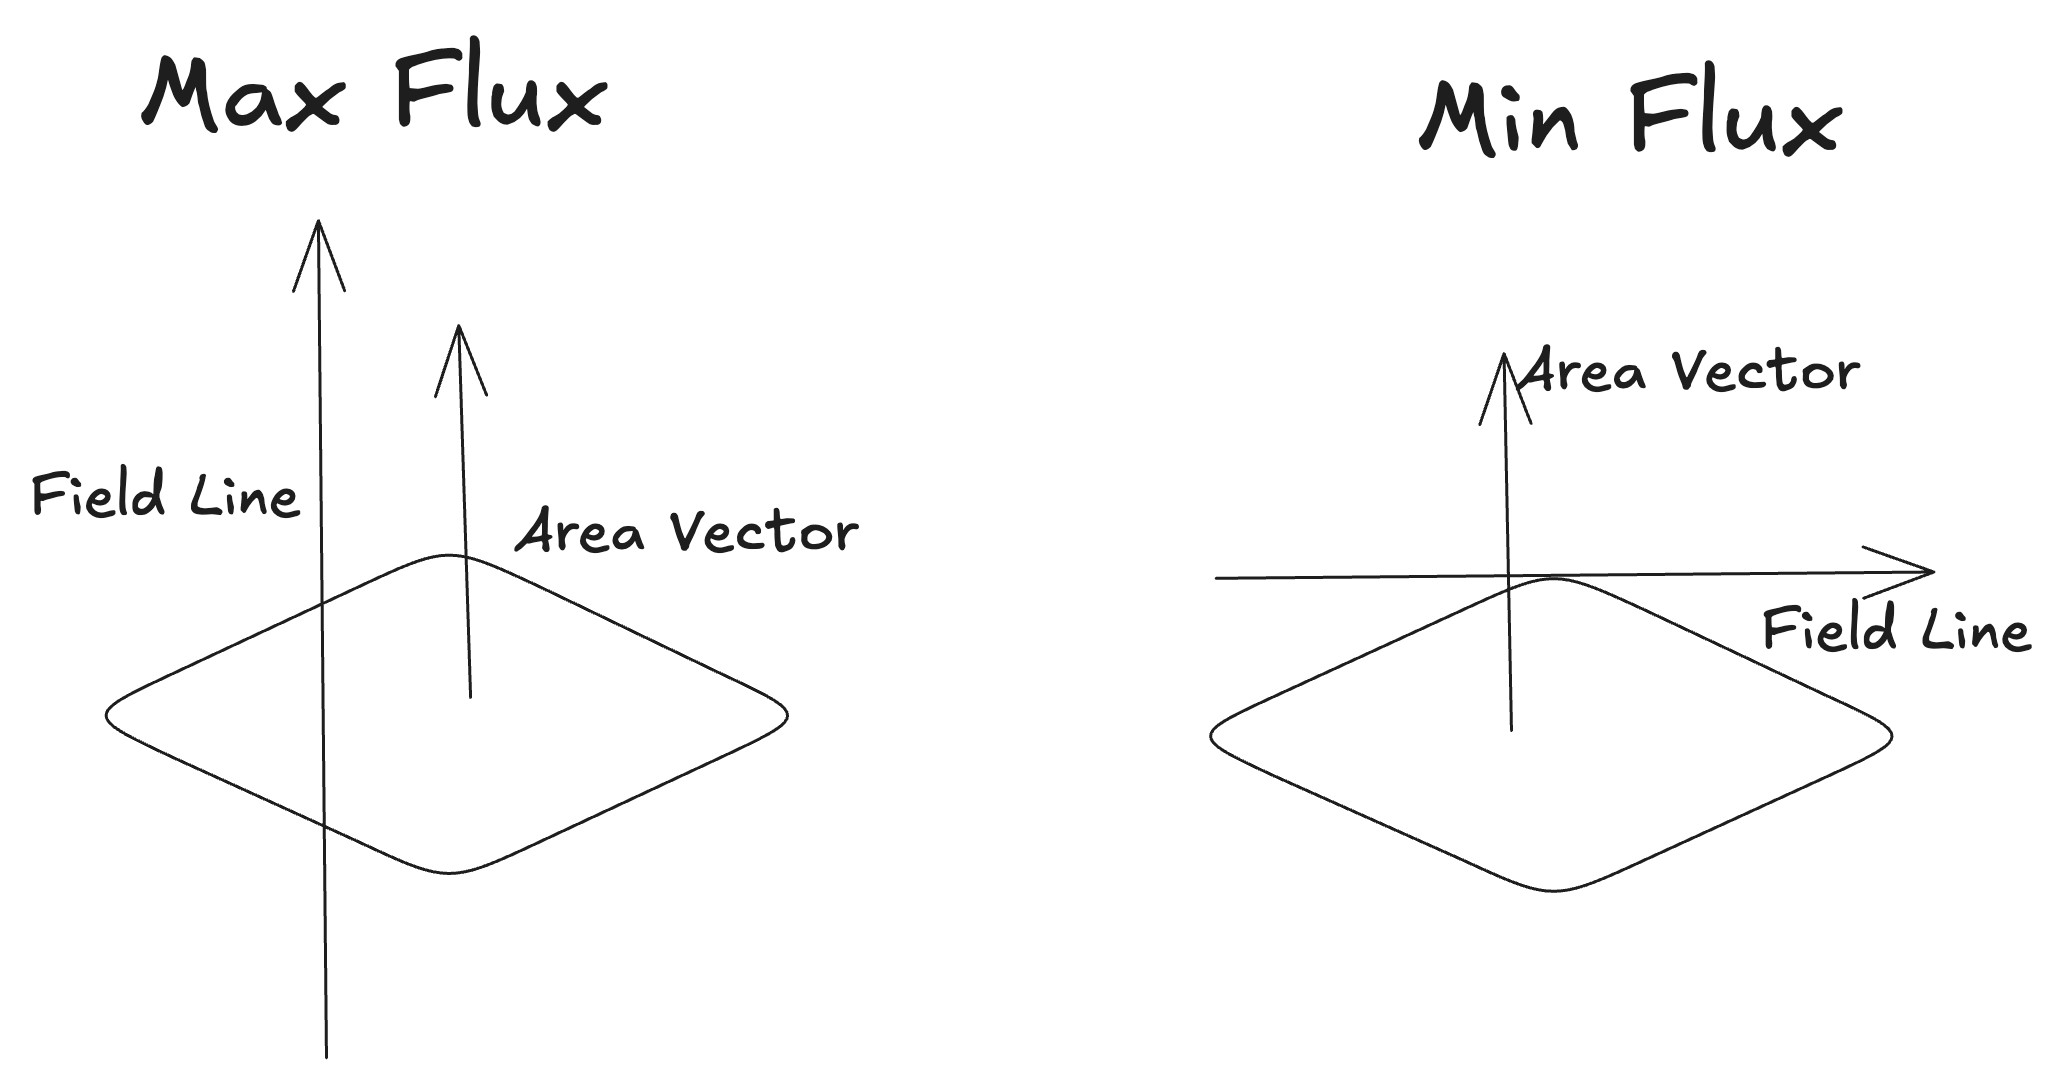
\includegraphics[width=0.5\textwidth]{figures/fluxamples.png}
    \caption{Visualization of max and min flux}
\end{figure}

Thus, you can compute the flux here:

$$\Phi = \vec{E} \cdot  \vec{A} = |\vec{E}||\vec{A}|\cos \theta $$

This is with the assumption that that
\begin{itemize}
    \item Plane is regular
    \item Field is constant
\end{itemize}

For an irregular plane / field, you can use this formula 

$$\Phi = \int \vec{E} \cdot \delta \vec{A}$$

\subsection{Closed Areas vs. Open Areas}

Gaussian Surfaces are closed figures, and that allows you to find a direction for the area vector, which is always outwards. Some additional points about close areas and flux:

\begin{itemize}
    \item The flux for an object that is hit by continious equipotentials and doesn't contain any of their own is zero
    \item For example, if you have flux that goes through a box, the flux is zero
\end{itemize}

\begin{figure}[H]
    \centering
    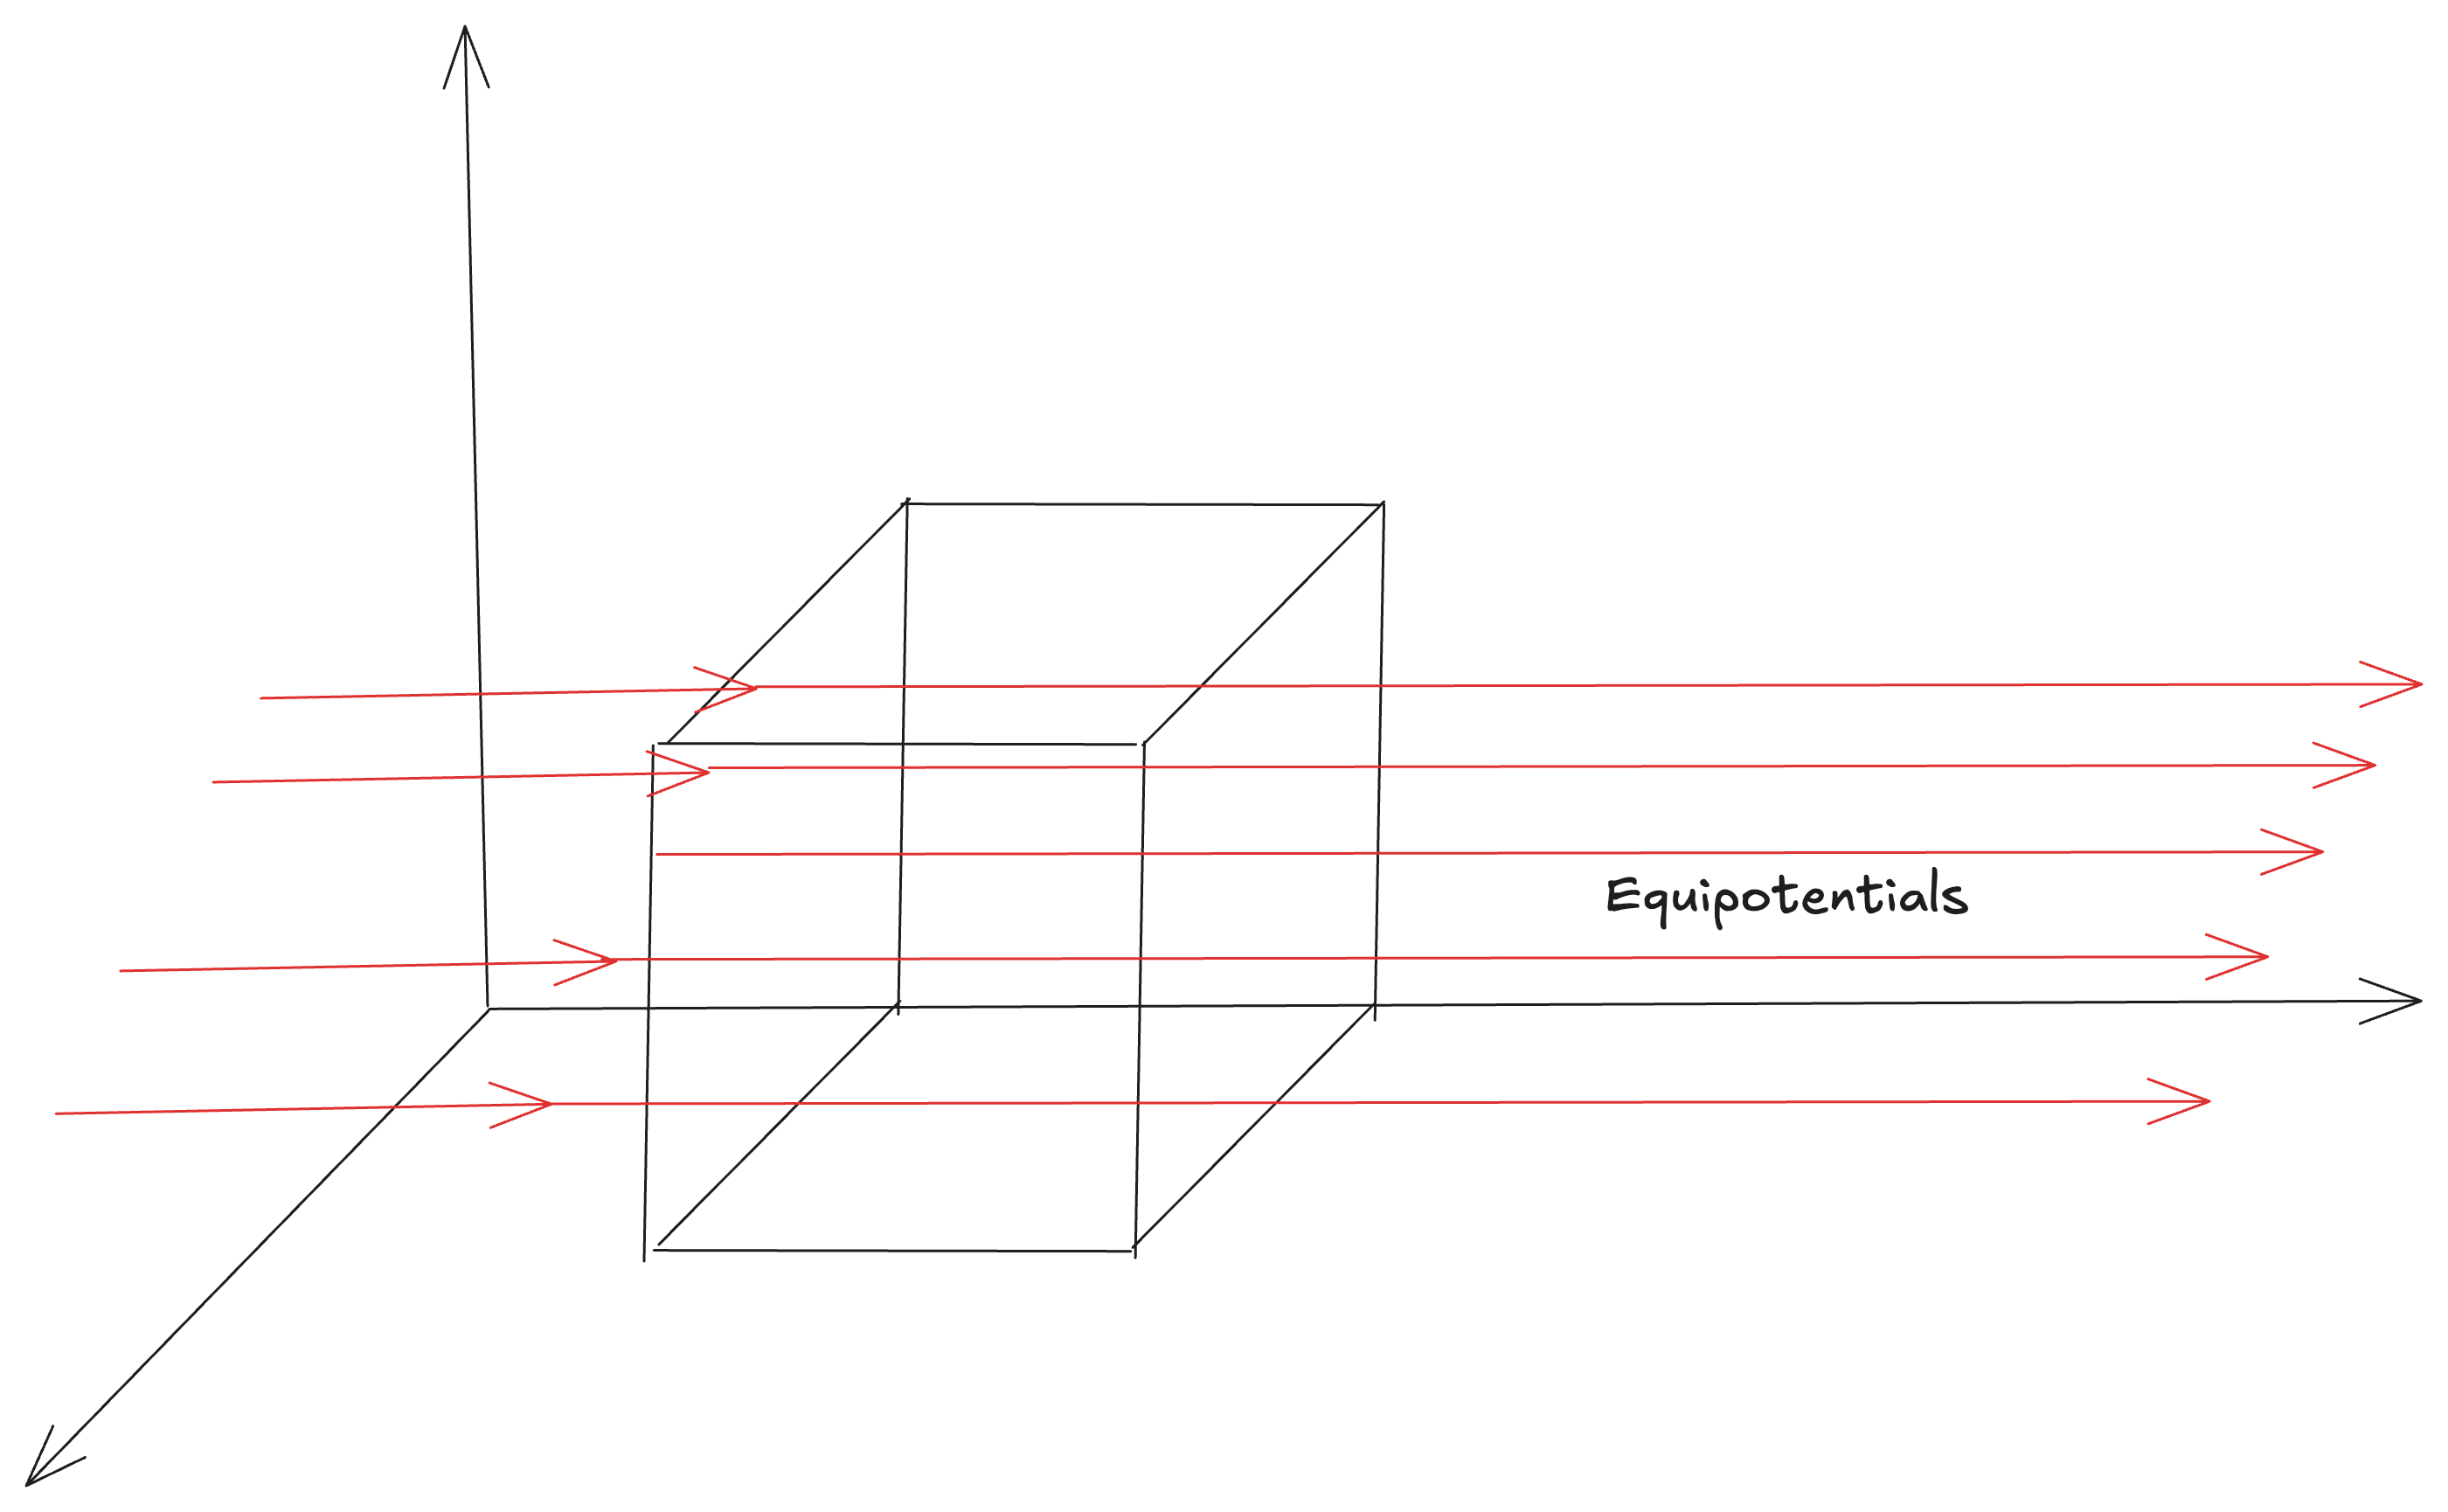
\includegraphics[width=0.3\textwidth]{figures/ExampleofEquipotentials.png}
    \caption{Object with zero flux}
\end{figure}

\end{document}